%%%%%%%%%%%%%%%%%%%%%%%%%%%%%%%%%%%%%%%%%%%%%%%%%%%%%%%%%%%%%%%%%
% Contents : The use of the reports chapter
% $Id : grisbi-manuel-reports.tex, v 0.4 2002/10/27 Daniel Cartron
% $Id : grisbi-manuel-reports.tex, v 0.5.0 2004/06/01 Loic Breilloux
% $Id : grisbi-manuel-reports.tex, v 0.6.0 2011/11/17 Jean-Luc Duflot
% $Id : grisbi-manuel-reports.tex, v 0.8.9 2012/04/27 Jean-Luc Duflot
% $Id : grisbi-manuel-reports.tex, v 1.0 2014/02/12 Jean-Luc Duflot
%%%%%%%%%%%%%%%%%%%%%%%%%%%%%%%%%%%%%%%%%%%%%%%%%%%%%%%%%%%%%%%%%

\chapter{États\label{reports}}


\section{Introduction\label{reports-intro}}


Grisbi vous permet de créer des états de comptabilité. Un état représente un statut actuel de vos comptes, formaté selon certains critères, entièrement choisis par l'utilisateur. Cela rend cette fonction entièrement personnalisable et très puissante.

% espace pour changement de thème
\vspacepdf{5mm}
Grisbi tient compte de toutes les données de votre fichier de comptes, y compris les archives. Vous pouvez choisir la période de temps, les comptes, les tiers, les catégories, les imputations budgétaires, les modes de règlement, le caractère rapproché ou non des opérations, les (sous-) opérations ventilées, etc. En fait toutes les informations décrivant une opération peuvent servir de \indexword{critère de \gls{tri}}\index{critère de tri}. Vous pouvez ensuite organiser hiérarchiquement l'affichage de l'état ainsi défini, par comptes, tiers, catégories ou imputations budgétaires, ajouter des séparations, et enfin afficher des libellés de données, des totaux ou sous-totaux au choix, et des données quelconques des opérations.

Par exemple, vous pouvez afficher la liste de toutes les dépenses d'un mois tous comptes confondus, ou toutes les opérations d'une catégorie sur une année, etc. Vous pouvez ajouter et enchaîner pratiquement autant de critères qu'il y a d'informations décrivant une opération, de façon à obtenir tous types de représentations imaginables.

% espace pour changement de thème
\vspacepdf{5mm}
L'onglet \menu{États} sert à créer des états et à mémoriser tous leurs paramètres, ce qui permet de les réafficher ultérieurement à la demande.

% espace pour changement de thème
\vspacepdf{5mm}
La liste des états existants s'affiche dans le panneau de navigation en cliquant sur le petit triangle à gauche de l'onglet \menu{États}. Tant que vous n'avez pas créé vous-même au moins un état, cette liste est vide.

\textbf{Note} : ces triangles peuvent être remplacés, en fonction du thème de l'environnement de bureau ou du gestionnaire de fenêtres que vous utilisez, par d'autres caractères tels que +, -, >, <, etc.

% espace pour changement de thème
\vspacepdf{5mm}
Pour avoir accès à la \indexword{gestion des états}\index{etats@états !gestion}, déroulez d'abord  la liste des états dans le panneau de navigation en cliquant sur le petit triangle, puis cliquez sur un des sous-onglets, ou déplacez-y la sélection avec les touches du clavier \key{Flèche Haut} \key{Flèche Bas}, \key{Page Haut} ou \key{Page Bas} ou avec la molette de la souris, ou encore, sélectionnez \menu{États} en cliquant sur l'un des deux petits triangles à gauche de la barre d'information, et faites défiler les différents items (voir le chapitre \vref{home}, \menu{Accueil}).

% espace pour changement de thème
\vspacepdf{5mm}

Le pavé des détails affiche deux éléments :
\begin{itemize}
	 \item la barre d'outils ;
	 \item l'état complet, si un état a été sélectionné.
\end{itemize}

% saut de page pour titre solidaire
\newpage


\section{Barre d'outils\label{reports-functions}}


La barre d'outils des états présente les fonctions suivantes  :

\begin{itemize}
	 \item \menu{Nouvel état} : ouvre une fenêtre comprenant la liste déroulante des états préformatés avec une description pour chacun d'eux ;
	 \item \menu{Importer} : permet d'importer un état contenu dans un fichier ;
	 \item \menu{Exporter} : permet d'exporter un état dans un fichier de format 	divers ;
	 \item \menu{Imprimer} : ouvre la fenêtre du gestionnaire d'imprimante et de 	ses options ;
	 \item \menu{Supprimer} : supprime l'état sélectionné ;
	 \item \menu{Propriétés} : affiche les paramètres de l'état sélectionné pour éventuellement les modifier, les améliorer ou les adapter ;
	 \item \menu{Cloner} : permet de faire une copie identique à l'état sélectionné.
\end{itemize}

La barre d'outils peut être déplacée dans l'écran en cliquant sur sa poignée (petit rectangle vertical à gauche de la barre) et en la déplaçant. Pour la réattacher à son emplacement d'origine dans le pavé des détails, la remettre en haut de la fenêtre, le haut de la poignée sur le petit  trait qui visualise sa place d'origine.


\section{Sélection d'un état\label{reports-selection}}


Pour sélectionner un état, vous avez deux moyens :

\begin{itemize}
	 \item dans le panneau de navigation, cliquez sur le nom de l'état, ou déplacez la sélection avec les touches du clavier \key{Flèche Haut} \key{Flèche Bas},  \key{Page Haut} ou \key{Page Bas} ou avec la molette de la souris ;
	 \item  dans la barre d'information, cliquez sur l'un des deux petits triangles à sa gauche pour faire défiler les différents états.
% saut de ligne pour indentation correcte de la note dans la liste

	 \textbf{Note} : ces triangles peuvent être remplacés, en fonction du thème de l'environnement de bureau ou du gestionnaire de fenêtres que vous utilisez, par d'autres caractères tels que +, -, >, <, etc.
\end{itemize}

 % espace avant Attention ou Note  : 5 mm
\vspacepdf{5mm}
	\textbf{Note} : les états ne peuvent être \indexword{listés}\index{etats@états !liste} que si la liste est déroulée dans le panneau de navigation.

 % espace avant Attention ou Note  : 5 mm
\vspacepdf{5mm}
\textbf{Note} : tant que vous n'avez pas créé vous-même au moins un état, cette liste est vide.
 % espace après Attention ou Note  : 5 mm
\vspacepdf{5mm}

Le nom de l'état apparaît alors dans la barre d'information, et, dans le panneau de navigation, sur fond bleu{\couleur}. Le contenu de l'état s'affiche dans le \ifIllustration pavé des détails\refimage{reports-display-img}.
\else pavé des détails.
\fi

\ifIllustration
\begin{figure}[ht]
\begin{center}
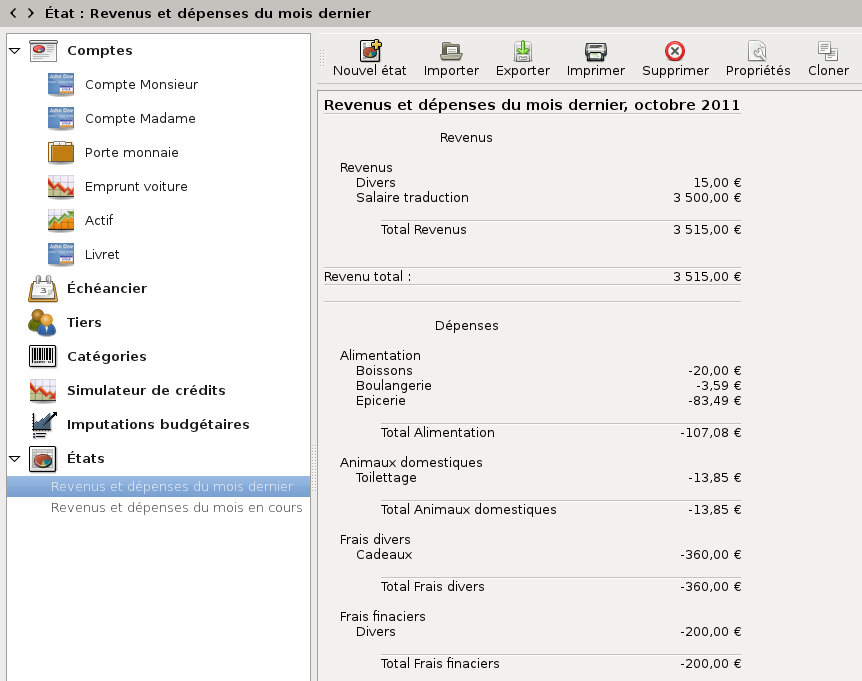
\includegraphics[scale=0.5]{image/screenshot/reports_display}
\end{center}
\caption{Onglet des états}
\label{reports-display-img}
\end{figure}
\fi

L'affichage se présente de la manière que vous avez définie au moment de la création de l'état. Il est toujours possible de le modifier (voir la section \vref{reports-modify}, \menu{Modification d'un état}).


\section{Les états préformatés}


Grisbi fournit par défaut plusieurs états préformatés que vous pouvez utiliser tels quels, ou bien comme base pour créer les vôtres. Ils sont accessibles à partir de la fonction \menu{Nouvel état} et sont les suivants :

\begin{itemize}
	\item \menu{Revenus et dépenses du mois dernier} ;
	\item \menu{Revenus et dépenses du mois en cours} ;
	\item \menu{Budget annuel} ;
	\item \menu{État vierge} : pour créer un état à partir de rien ;
	\item \menu{Remise de chèques} : pour faire un état sur tous les chèques encaissés ;
	\item \menu{Dépenses mensuelles par tiers} ;
	\item \menu{Recherche} : pour faire des recherches d'opération.
\end{itemize}


\section{Création d'un nouvel état}


Pour créer un nouvel état, consultez le chapitre \vref{reportscreation}, \menu{Création d'un état}. La procédure complète de création d'un état et de sa personnalisation est explicitée en détail dans les différentes sections de ce chapitre.


\section{Modification d'un état\label{reports-modify}}


Pour modifier un état, procédez comme suit :

\begin{enumerate}
	 \item sélectionnez-le dans le panneau de navigation ou avec la barre d'information ;
	 \item cliquez sur l'outil \menu{Propriétés} dans la barre d'outils ;
	 \item la fenêtre de création/modification s'ouvre, la même que celle utilisée pour la création d'un état ; vous pouvez y modifier ou y ajouter tous les paramètres relatifs à un état ;
	 \item validez.
\end{enumerate}

La modification peut se ramener à changer le compte pour lequel vous voulez établir cet état, mais elle peut aussi représenter quelque chose de beaucoup plus complexe. Pour plus de précisions, voir la section \vref{reportscreation-selection}, \menu{Sélection des données}.


\section{Clonage d'un état}


Pour cloner un état, procédez comme suit :

\begin{enumerate}
	 \item sélectionnez-le dans le panneau de navigation ou avec la barre d'information ;
	 \item cliquez sur l'outil \menu{Cloner} dans la barre d'outils ;
	 \item la fenêtre de création/modification s'ouvre, la même que celle utilisée pour la création d'un état ; vous pouvez y modifier ou y ajouter tous les paramètres relatifs à un état ;
	 \item validez.
\end{enumerate}

Grisbi duplique intégralement l'état d'origine, y compris son nom ; le clone de l'état apparaît en grisé à la fin de  la liste des états dans le panneau de navigation ; la première chose que vous devrez faire sera de lui donner un nouveau \indexword{nom}\index{etat@état !nommer} (voir la section \vref{reportscreation-display-general}, \menu{Généralités}). 


\section{Suppression d'un état\label{reports-delete}}


Pour supprimer un état, procédez comme suit :

\begin{enumerate}
	 \item sélectionnez-le dans le panneau de navigation ou avec la barre d'information ;
	 \item cliquez sur l'outil \menu{Supprimer} dans la barre d'outils, ou cliquez-droit dans le panneau de navigation sur l'état concerné et sélectionnez \menu{Supprimer cet état} ;
	 \item une  boîte de dialogue s'ouvre et vous demande la confirmation ou l'annulation de cette suppression.
\end{enumerate}

\strong{Attention} : si vous validez la suppression, l'état sera détruit irrémédiablement ; cette opération est \indexword{irréversible}\index{opération !irréversible}.


\section{Import et export\label{reports-importexport} }


En plus des états préformatés et de ceux que vous pouvez créer vous-même, Grisbi vous permet d'exporter ou d'importer des états créés dans un autre fichier de comptes.

%De plus, une bibliothèque d'états sera disponible sous peu sur le site de
%Grisbi.


\subsection{Import d'un état\label{reports-importexport-import} }

Pour importer un état, procédez comme suit :

\begin{enumerate}
	 \item cliquez sur l'outil \menu{Importer} dans la barre d'outils : une fenêtre de gestionnaire de fichiers s'affiche ;
	 \item choisissez le répertoire et le nom du fichier à importer, dont l'\indexword{extension} doit être \file{.egsb}\index{extension !.egsb} ;
	 \item cliquez sur le bouton \menu{Ouvrir} ; 
	 \item une boîte d'informations s'affiche ; lisez attentivement les avertissements ou instructions, puis cliquez sur le bouton \menu{Fermer} ;
	 \item l'état importé est listé dans le panneau de navigation ; suivez éventuellement les instructions qui viennent de vous être données.
\end{enumerate}

\strong{Attention} : d'une manière générale, il est déconseillé d'avoir des accents ou des espaces dans les noms des répertoires et fichiers utilisés par Grisbi. Si c'est le cas, renommez-les maintenant. Par exemple, les espaces peuvent être remplacées par des tirets bas (\_).
 % espace après Attention ou Note  : 5 mm
\vspacepdf{5mm}

Vous pouvez ensuite personnaliser le nouvel état importé. Il est probable que vous ayez au moins à vérifier si le nom des comptes sélectionnés est correct.


\subsection{Export d'un état\label{reports-importexport-export} }

Pour exporter un état, procédez comme suit :

\begin{enumerate}
	 \item sélectionnez l'état dans le panneau de navigation ou avec la barre d'information ;
	 \item  cliquez sur l'outil \menu{Exporter} dans la barre d'outils : une fenêtre de gestionnaire de fichiers s'affiche ;
	 \item par défaut, le nom du fichier à exporter est celui de l'état ;
	modifiez-le éventuellement et sélectionnez le format du fichier désiré (son extension) ;
	 \item choisissez son répertoire de destination ;
	 \item cliquez sur le bouton \menu{Enregistrer}.
\end{enumerate}

\textbf{Note} : le format du fichier est par défaut le format des pages web (\indexword{.html})\index{extension !.html}, mais on peut choisir aussi le format natif de Grisbi (\indexword{.egsb})\index{extension !.egsb}, ou encore un format de texte (\indexword{\gls{CSV}})\index{extension !.csv}.
 
 % espace après Attention ou Note  : 5 mm
\vspacepdf{5mm}

Dans le cas d'une exportation en format \indexword{\gls{HTML}}\index{html}, le fichier est conforme à la norme XHTML 1.0, ce qui devrait garantir son bon affichage par les navigateurs modernes.  Il est également encodé en Unicode, ce qui peut causer des problèmes auprès des navigateurs web qui ne sont pas configurés correctement pour auto-détecter le contenu d'une page web.


\section{Impression d'un état\label{reports-print}}


Pour imprimer un état, procédez comme suit :

\begin{enumerate}
	 \item sélectionnez-le dans le panneau de navigation ou avec la barre d'information ;
	 \item cliquez sur le bouton \menu{Imprimer} de la barre d'outils. Une fenêtre d'impression s'ouvre, dont l'aspect et les fonctions dépendent de votre gestionnaire d'impression ; vous aurez le plus souvent les choix suivants :
		  \begin{itemize}
			  \item imprimer dans un fichier (en format \indexword{\gls{PostScript}}\index{postscript}, \indexword{\gls{PDF}}\index{pdf} ou \indexword{\gls{SVG}}\index{svg}),
			  \item imprimer avec votre imprimante.
		  \end{itemize}
\end{enumerate}

En fonction de votre gestionnaire d'impression, vous pourrez disposer de réglages divers tels que la taille et l'orientation de la feuille, la résolution, la police d'impression et sa taille, etc.











